\subsection{The Swelling and Permeability of T4 Salt Clay}
\label{sec:t4swell}
\Authors{Mathias Nest, Till Popp (IfG)}

\begin{figure}[ht]
\centering
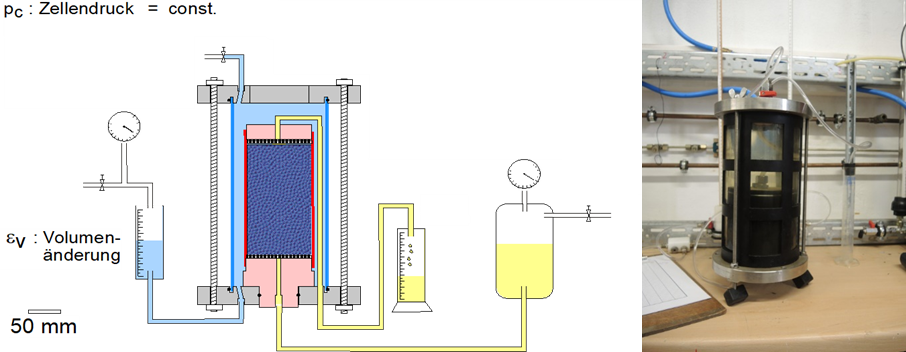
\includegraphics[width=0.9\textwidth]{figures/IfG-T4-Perm-aufbau.png}
\caption{Setup of the experiment to measure the closure of pathways in clay through
swelling.}
\label{fig:t4swellsetup}
\end{figure}

The transport properties of a material depend not only on the pore space, but also on the permeability, which is the decisive measure for the hydraulic integrity of a material. We measure the permeability based on the Darcy equation, which takes into account the pressure difference, the viscosity of the fluid, and a geometry factor of the sample.
\index{Darcy equation}

For the present project the permeability was measured under stationary stress/pressure conditions using a saturated brine solution. The setup that we used was build at the IfG, and is shown in Figure \ref{fig:t4swellsetup}. The mantle of the cylindric samples were covered with rubber cuffs, and filter plates on top and below. Thus they are isolated from the medium (water) which provides the cell pressure. The amount of brine that passes through the sample is measured as a function of time, so that the permeability and its change can be calculated. 

%---------------------------------------------------------------------------------------------------
%\subsection{Oedometer Test (BGR)}
%---------------------------------------------------------------------------------------------------

\subsection{The Wetting and Drying Paths of the Opalinus Claystone}
\label{sec:Shrinkage_Swelling_Exp}
\Authors{Amir Shoarian Sattari (CAU)}

The shrinkage and swelling of claystone results in micro fracking and higher permeability values, which in nuclear waste disposal sites can lead to contamination of groundwater. Micro fracking also decreases the strength of the material subjected to THM  loading processes. Typically, the swelling pressure and heave of claystone is determined using Oedometer tests \cite{Peronetal2009}, where a constrained or unconstrained sample is subjected to the swelling process (Figure \ref{fig:Amir_Shrinkage_Swelling_Setup}). During the test procedure, the swelling pressure, as well as the heave magnitude, are recorded. It is observed that the swelling pressure in sandy facies of claystone is lower than shaly facies. In contrast to the swelling tests, shrinkage tests are less common and are complicated to perform on rock materials. \cite{Minardietal2016} performed a shrinkage test on claystone with shaly and sandy facies using a desiccator and various salt solutions (Figure  \ref{fig:Amir_Shrinkage_Minardi}). During the test procedure the axial strain values obtained from the strain gauges, as well as sample weight, are measured.
\index{Oedometer test}

\begin{figure}[!ht]
\begin{subfigure}[c]{0.48\textwidth}
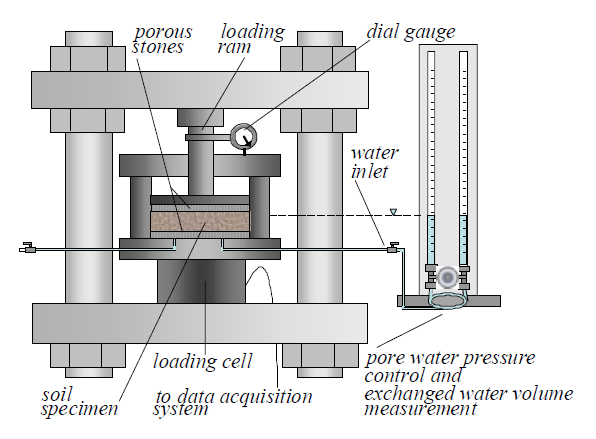
\includegraphics[width=1\textwidth]{figures/Amir_Shrinkage_Swelling_Setup.png}
\subcaption{}
\label{fig:Amir_Shrinkage_Swelling_Setup}
\end{subfigure}
\hfill
\begin{subfigure}[c]{0.48\textwidth}
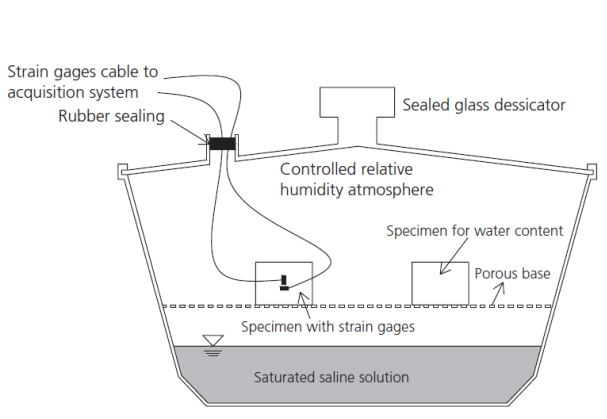
\includegraphics[width=1\textwidth]{figures/Amir_Shrinkage_Minardi.png}
\subcaption{}
\label{fig:Amir_Shrinkage_Minardi}
\end{subfigure}
\caption{The swelling and shrinkage tests on Opalinus claystone (a) the Oedometer test setup for constrained swelling pressure in Opalinus clay samples \cite{Peronetal2009}, and (b) measuring the drying and wetting paths using desiccator \cite{Minardietal2016}}
\end{figure}

Two prepared thin cylindrical sections of sandy Opalinus claystone (Mont Terri) with a dimension of 100x10 $mm (DxH)$ are used to determine the anisotropy in shrinkage and swelling behavior of claystone. Due to the mineral structure of claystone and its layering orientation, the anisotropy factor has a significant influence on the direction of shrinkage and swelling as well as the micro fracking formation. The initial sample is used to determine the axial strains in parallel and perpendicular directions to the layering orientations. The strain gauge strips (HBM, $LY 10 (mm)$/120 $\Omega$) are glued and attached to the surface of the sample. The second sample is used to measure the weight change in the sample under different salt solutions. The saturated salt solutions are located inside the desiccator and will result in osmotic suction and eventually in the wetting and drying of the samples. The total suction($\psi_\text{total}$) value can be measured using the Kelvin’s relation, which is derived from ideal gas law:
\index{ideal gas law}

\begin{equation}
\label{eq:Total_Suction}
\psi_\text{total} = \frac{RT}{V_\text{mol}} \ln(\frac{P_\text{vap}^{cur}}{P_\text{vap}^{cur=0}})
\end{equation}

where, $(\frac{P_\text{vap}^{cur}}{P_\text{vap}^{cur=0}})$ is the relative humidity, $P_\text{vap}^{cur=0}$ is the vapor pressure when the surface curvature is equal to zero (flat surface), $R$ is the universal gas constant, $T$ is the temperature and $V_\text{mol}$ is the molecular volume of water. The equilibrium inside the desiccator is reached when the strain gauges value or water content of the samples are constant in two consecutive readings. The results obtained from the drying and wetting paths of the Opalinus claystone are given in \ref{sec:mex06}, where a numerical simulation and comparison to the experimental data are provided. The test procedure is time consuming and after measuring the data for more than 120 days, the applied suction and water content percentages are calculated and plotted. 

%---------------------------------------------------------------------------------------------------
\subsection{In-situ Condition Desiccation Process}

Topology, respectively morphology investigations of fractures induced in clay stone throughout drying processes require a number of experimental sequences ranging from the drying process itself to characterization of the induced fractures by X-Ray Computed Tomography. The required samples are prepared and characterized by the University of Kiel with a dimension of radius $r=5 \, \text{mm}$ and height $h=50 \, \text{mm}$ to guarantee the realization of scans in Regions of Interests (RoIs) down to a characteristic edge length of $6 \, \text{mm}$ resulting in a resolution of 2 micrometers per voxel.
\index{drying}
\index{XRCT application}

Two different experimental set-ups are planned; nevertheless the first proposed experimental implementation is preferred over the second.

\subsubsection*{Drying Wet Samples - From Wet to Dry}

Saturated samples are prepared by the University of Kiel and submerged in a shrink tube in order to minimize the change of the desired state. Once the experiments are performed on the sample the shrink tube is removed and the probe is installed in an uni-axial testing device. The sample is installed in a heat chamber and loaded by an axial force of $f_\text{ax} = 500 \, \text{N}$/, resulting in an axial stresses of $\sigma_\text{ax} = 0.25 \text{MPa}$ (potentially up to $f_{ax} = 5 \, \text{kN}$/$ \sigma_\text{ax} = 2.5 \text{MPa}$) while axial deformations are measured under controlled temperature conditions. By measuring the sample's weight at characteristic states (twice - beginning and end) the volumetric deformations can be determined and related to the change of saturation. The sample characterization is then completed by XRCT scans to determine the features of the induced fractures. Finally the stiffness degradation is determined by ultrasound experiments measuŕing the P-wave run times at 2, respectively 6 MHz.

\subsubsection*{Wetting dry Samples - From Dry to Wet}

Since it is extremely time consuming to increase the saturation of the sample this second setting is only an alternative to the introduced set-up in case the first experiment fails. The set-up is comparable to the proposed experiment but performed in a heat-humidity chamber at rel. humidity between 10 - 90 \% and temperatures between $5-90^\circ C$. The applied axial Force would reduce to $f_\text{ax}=50 \, \text{N}$.